\documentclass{minimal}
\usepackage[T1]{fontenc}
\usepackage{newtxtext}
\usepackage{newtxmath}
\usepackage{xcolor}
\usepackage{tikz}

\pdfpagewidth=500pt
\pdfpageheight=650pt
\setlength{\paperwidth}{500pt}
\setlength{\paperheight}{650pt}
\setlength{\textwidth}{500pt}
\setlength{\textheight}{650pt}
\setlength{\oddsidemargin}{-72pt}
\setlength{\topmargin}{-72pt}
\setlength{\headheight}{0pt}
\setlength{\headsep}{0pt}
\setlength{\footskip}{0pt}
\setlength{\parindent}{0pt}
\pagestyle{empty}

\definecolor{tsblue}{HTML}{356787}
\definecolor{tspurple}{HTML}{635694}
\definecolor{tsgray}{HTML}{66717C}
\definecolor{tslight}{HTML}{C8CDD2}
\definecolor{tsink}{HTML}{202833}

\newcommand{\panel}[4]{%
  \draw[rounded corners=8pt,draw=tslight,line width=1pt,fill=white]
    (#1,#2) rectangle (#3,#4);
}
\newcommand{\tick}[3]{%
  \draw[draw=tsink,line width=.8pt] (#1,#2-3) -- (#1,#2+3);
  \node[anchor=north,font=\fontsize{15}{17}\selectfont,text=tsink]
    at (#1,#2-5) {#3};
}
\newcommand{\ci}[6]{%
  \draw[draw=#1,line width=1.7pt] (#3,#2) -- (#4,#2);
  \draw[draw=#1,line width=1.1pt] (#3,#2-4) -- (#3,#2+4);
  \draw[draw=#1,line width=1.1pt] (#4,#2-4) -- (#4,#2+4);
  \filldraw[draw=#1,fill=#6,line width=1.2pt] (#5,#2) circle (4pt);
}

\begin{document}
\begin{tikzpicture}[x=1pt,y=1pt,line cap=round,line join=round]
\useasboundingbox (0,0) rectangle (500,650);
\fill[white] (0,0) rectangle (500,650);

% (a) Q2 load-bearing effects.
\panel{10}{440}{490}{640}
\node[anchor=north west,font=\bfseries\fontsize{20}{23}\selectfont,text=tsink]
  at (22,630) {(a) Q2 forecast skill removed ($\Delta R^2$)};
\filldraw[draw=tsblue,fill=tsblue] (176,600) circle (4pt);
\node[anchor=west,font=\fontsize{16}{18}\selectfont] at (187,600)
  {state ablation};
\filldraw[draw=tsgray,fill=white,line width=1.2pt] (326,600) circle (4pt);
\node[anchor=west,font=\fontsize{16}{18}\selectfont] at (337,600)
  {$T\!\rightarrow I$};
\node[anchor=east,font=\fontsize{18}{20}\selectfont,text=tsink]
  at (142,560) {Validation};
\node[anchor=east,font=\fontsize{18}{20}\selectfont,text=tsink]
  at (142,492) {Temporal shift};
\draw[draw=tslight,line width=1pt] (158.89,458) -- (158.89,585);
\ci{tsblue}{568}{216.04}{389.11}{258.53}{tsblue}
\ci{tsgray}{552}{228.40}{398.53}{264.80}{white}
\ci{tsblue}{500}{285.29}{427.60}{336.40}{tsblue}
\ci{tsgray}{484}{301.91}{444.40}{351.69}{white}
\draw[draw=tsink,line width=1pt] (150,455) -- (470,455);
\tick{158.89}{455}{0.00}
\tick{247.78}{455}{0.01}
\tick{336.67}{455}{0.02}
\tick{425.56}{455}{0.03}

% (b) Q3 weather-control effects.
\panel{10}{226}{490}{423}
\node[anchor=north west,font=\bfseries\fontsize{20}{23}\selectfont,text=tsink]
  at (22,413) {(b) Q3 loss increase under control weather};
\node[anchor=east,font=\fontsize{18}{20}\selectfont,text=tsink]
  at (142,350) {Matched control};
\node[anchor=east,font=\fontsize{18}{20}\selectfont,text=tsink]
  at (142,282) {Normalized mean};
\draw[draw=tslight,line width=1pt] (161.67,245) -- (161.67,385);
\ci{tspurple}{350}{180.33}{228.17}{204.50}{tspurple}
\ci{tspurple}{282}{252.83}{457.67}{349.33}{tspurple}
\draw[draw=tsink,line width=1pt] (150,242) -- (470,242);
\tick{161.67}{242}{0.000}
\tick{245.00}{242}{0.005}
\tick{328.33}{242}{0.010}
\tick{411.67}{242}{0.015}

% (c) Forecast scores on the same Q3 subset.
\panel{10}{8}{490}{207}
\node[anchor=north west,font=\bfseries\fontsize{20}{23}\selectfont,text=tsink]
  at (22,197) {(c)};
\filldraw[draw=tspurple,fill=tspurple] (126,188) circle (4pt);
\node[anchor=west,font=\fontsize{15}{17}\selectfont] at (137,188) {Actual};
\filldraw[draw=tsgray,fill=tsgray] (240,188) circle (4pt);
\node[anchor=west,font=\fontsize{15}{17}\selectfont] at (251,188) {Matched};
\filldraw[draw=tsink,fill=tslight] (371,188) circle (4pt);
\node[anchor=west,font=\fontsize{15}{17}\selectfont] at (382,188) {Mean};

\draw[draw=tsink,line width=1pt] (100,135) -- (465,135);
\tick{156.15}{135}{0.54}
\tick{268.46}{135}{0.58}
\tick{380.77}{135}{0.62}
\filldraw[draw=tspurple,fill=tspurple] (395.96,157) circle (4.5pt);
\filldraw[draw=tsgray,fill=tsgray] (294.96,157) circle (4.5pt);
\filldraw[draw=tsink,fill=tslight] (164.62,157) circle (4.5pt);
\node[anchor=north,font=\fontsize{18}{20}\selectfont,text=tsink]
  at (282.5,105) {$R^2$ on Q3 subset};

\draw[draw=tsink,line width=1pt] (100,59) -- (465,59);
\tick{156.15}{59}{0.15}
\tick{268.46}{59}{0.17}
\tick{380.77}{59}{0.19}
\filldraw[draw=tspurple,fill=tspurple] (151.66,81)
  rectangle ++(8pt,8pt);
\filldraw[draw=tsgray,fill=tsgray] (203.35,81)
  rectangle ++(8pt,8pt);
\filldraw[draw=tsink,fill=tslight] (420.77,81)
  rectangle ++(8pt,8pt);
\node[anchor=north,font=\fontsize{18}{20}\selectfont,text=tsink]
  at (282.5,29) {RMSE on Q3 subset};

\end{tikzpicture}
\end{document}
